\documentclass{article}

\usepackage{../../austin137}
\usepackage{../../local}
\usepackage{chemformula}
\usehyperstuff

\def\OCO{$\ch{CO_2}$}
\def\reviewpart{\textbf{Review} (\emph{Not for Credit})\ \ }				%	Extra Part on Questions
\newcommand{\I}{\mathbbold 1}

\usepackage{wrapfig}

\begin{document}

%%%%%%%%%%%%%%%%%%%%%%%%%%%%%%%%%%%%%%%%%%%%%%%%%%%%%%%%%%%%%%%%%%%%%%%%%%%%%%%%
\addcopyright
\begin{center}
{\bf \large Physics W89 - Introduction to Mathematical Physics - Summer 2023}\\\medskip
{\bf \large Problem Set - Module 05 - The Eigentopic} \\\medskip
{\emph{Last Update: \today}\\}
{ Student: Yutong Du}
\end{center}


\dphline\bigskip
%%%%%%%%%%%%%%%%%%%%%%%%%%%%%%%%%%%%%%%%%%%%%%%%%%%%%%%%%%%%%%%%%%%%%%%%%%%%%%%%
\section*{Problem 5.1 - A Wee Quadratic Form Problem}
\relevid{Quadratic Forms}

\paragraph{}
In this problem we will deal with \emph{real} vector spaces and matrices only.
Let $Q(x_{1},\cdots,x_{n})$ be a quadratic form (a homogenous degree-2 polynomial in the variables $x_{1}, \cdots x_{n}$).  
We can write this in matrix language by defining the vector $\vec{x}$ and a symmetric $(n\times n)$ matrix $\mathsf{Q}$ such that 
	\begin{equation}
		\vec{x} \equiv \smmatrix{0.8}{x_{1}\\\vdots\\x_{n}},	\qquad Q(x_{1},\cdots,x_{n}) = \vec{x}\cdot\mathsf{Q}\vec{x} = \vec{x}^{\T}\mathsf{Q}\vec{x}.
	\label{quadratic}
	\end{equation}
The components of the symmetric matrix $\mathsf{Q}$ can be found via
	\begin{equation}
		Q^{i}_{\,j} = \frac{1}{2}\frac{\partial^{2}Q}{\partial{x_{i}}\partial{x_{j}}}.
	\label{components}
	\end{equation}
Consider a two-degree-of-freedom system with $\vec{x} =\twovect{x_{1}}{x_{2}}$ and quadratic form $Q(x_{1},x_{2}) = ax_{1}^{2} + 2bx_{1}x_{2}+cx_{2}^{2}$.

%%%%%%%%%%%%%%%%%%%%%
\paragraph{(a)}
Find the matrix $\mathsf{Q}$ using Eq.~\ref{components} and show that $\vec{x}\cdot\mathsf{Q}\vec{x}$ gives the correct function $Q(x_{1},x_{2})$.

\begin{solution}
	This problem just involves us taking derivatives:
	\begin{align*}
		Q^1_1 &= \frac{1}{2}\pdv[2]{Q}{x_1} = \frac{1}{2}(2a) = a\\
		Q^1_2 &= \frac{1}{2}\pdv{Q}{x_1}{x_2} = \frac{1}{2}\pdv{x_2} \pdv{Q}{x_1} = b\\
		Q^2_1 &= Q^1_2 = b\\
		Q^2_2 &= \frac{1}{2}\pdv[2]{Q}{x_2} = \frac{1}{2}(2c) = c
	\end{align*}
	Therefore the matrix $Q$ is:
	\[
		Q = \begin{pmatrix} a & b\\ b& c \end{pmatrix} 
	\] 
	The only thing of note here is that $Q^1_2 = Q^2_1$ because we know that partial derivatives can be 
	swapped at no cost. Now we compute $\vec x^\T Q \vec x$: 
	\begin{align*}
		\vec x^\T Q \vec x &= \begin{pmatrix} x_1 & x_2 \end{pmatrix} \begin{pmatrix} a & b\\
	 b & c\end{pmatrix} \begin{pmatrix} x_1 \\x_2 \end{pmatrix} \\
				&= \begin{pmatrix} x_1 & x_2 \end{pmatrix}\begin{pmatrix} ax_1 + bx_2\\
				bx_1 + cx_2 \end{pmatrix} \\
				&= ax_1^2 + bx_1 x_2 + bx_1x_2 + cx_2^2\\
				&= ax_1^2 + 2bx_1x_2 + cx_2^2 
	\end{align*}
	which is exactly the equation $Q(x_1, x_2)$ from earlier. 
\end{solution}
\phline
%%%%%%%%%%%%%%%%%%%%%
\paragraph{}
We don't \emph{have} to restrict $\mathsf{Q}$ to be a symmetric matrix, but the symmetric part of $\mathsf{Q}$ is the only thing that will contribute to the quadratic form.

\paragraph{(b)}
Write down the most general $(2\times 2)$ real antisymmetric matrix $\mathsf{R}$ and show that $\vec{x}\cdot\mathsf{R}\vec{x} = 0$.  Also argue that using
Eq.~\ref{components} to find $\mathsf{Q}$ will only ever give rise to symmetric matrices.

\begin{solution}
	The most general asymmetric matrix is of the form: 
	\[
		R = \begin{pmatrix} 0 & a \\ -a & 0 \end{pmatrix} 
	\] 
	therefore we can now do the matrix multiplication:
	\begin{align*}
		\vec x^\T R \vec x &= \begin{pmatrix} x_1 & x_2  \end{pmatrix} 
		\begin{pmatrix} 0 & a \\ -a & 0 \end{pmatrix} \begin{pmatrix} x_1 \\ x_2 \end{pmatrix} \\
						  &= \begin{pmatrix} x_1 & x_2 \end{pmatrix} 
						  \begin{pmatrix} ax_2 \\ -ax_1 \end{pmatrix}  \\
						  &= ax_1x_2 - ax_2x_1  \\
						  &=  0 
	\end{align*}
	as expected. 
\end{solution}

%%%%%%%%%%%%%%%%%%%%%
\paragraph{(c)}
To generalize part (b), let $\mathsf{M}$ be an arbitrary real $(n\times n)$ matrix and let $\mathsf{Q}$ and $\mathsf{R}$ be the symmetric and antisymmetric parts of $\mathsf{M}$, respectively.  
Show that $\vec{x}^{\T}\mathsf{M}\vec{x} = \vec{x}^{\T}\mathsf{Q}\vec{x}$.
\spoilers{Try using index notation for the combination $\vec{x}^{\T}\mathsf{R}\vec{x}$.  What happens to your expression if you apply the antisymmetry of $\mathsf{R}$?}


\begin{solution}
	We know we can decompose the product into:
	\[
	\vec x^\T M \vec x = \vec x^\T( Q + R) \vec x = \vec x^\T Q \vec x + \vec x^\T R \vec x
	\] 
	Therefore, in order to show that $\vec x^\T M \vec x = \vec x^\T Q \vec x$, we need to show that $\vec x^\T
	R \vec x = 0$, so that the desired equality may be established. We can do so with the help of index 
	notation: 
	\[
	\vec x^\T R \vec x = x^j R^i_j x_i 
	\] 
	Now we can transpose this by swapping the row and column indices. In doing so, we use the fact that 
	$R^i_j = -R^j_i$, so therefore the expression flips sign when we do this:
	\[
	x^j R^i_j x_i = (-x_jR^j_i x^i)^\T
	\] 
	Now we reverse the transposition:
	\[
	x^j R^i_j x_i = -x^j R^i_j x_i
	\] 
	But now we've just shown that something is equal to the negative of itself, hence it must equal zero. Hence,
	the asymmetric part contributes nothing to the summation, and we conclude that $\vec x^\T M \vec x = 
	\vec x^\T Q \vec x$. 
\end{solution}
\bigskip
\dphline
\pagebreak
%%%%%%%%%%%%%%%%%%%%%%%%%%%%%%%%%%%%%%%%%%%%%%%%%%%%%%%%%%%%%%%%%%%%%%%%%%%%%%%%
\section*{Problem 5.2 - Carbon Dioxide (\OCO)}
\relevid{The Eigenvalue Problem;
Finding Eigenvalues;
Finding Eigenvectors}

\paragraph{}
	%~~~~~~~~~~~~~~ FIGURE ~~~~~~~~~~~~~~%
	\setlength{\intextsep}{0pt}%
	\begin{wrapfigure}[4]{r}{0cm}
		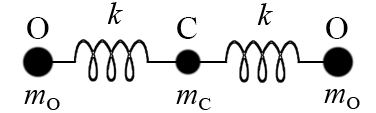
\includegraphics[width = 0.3\textwidth]{89-PS5-P2-CO2}
	\end{wrapfigure}
	%~~~~~~~~~~~~~~ FIGURE ~~~~~~~~~~~~~~%
Let's model a carbon dioxide molecule as three masses attached to two springs, as shown to the right. 
Let $x_{1}$ be the position of the left-most oxygen, $x_{2}$ be the position of the carbon with respect to its equilibrium position, and $x_{3}$ be the position of the 
right-most oxygen with respect to its equilibrium position.  
The two springs represent the carbon-oxygen double bond and each have identical spring constants $k$.\footnote{For this bond, $k \approx 843\ \units{N}/\units{m}$.}  
Let $m_{o}$ be the mass of an oxygen atom and $m_{c}$ be the mass of a carbon atom.

\paragraph{}
The configuration of our \OCO\ may be described as a vector.  Let's introduce the basis $\{\hat{e}_{1},\hat{e}_{2},\hat{e}_{3}\}$, where
the three unit vectors represent a unit displacement from the equilibrium position for the left oxygen, the central carbon, and the right oxygen, respectively.  
A general displacement of our carbon dioxide may be written as
	\begin{equation*}
		\vec{x} = x_{1}\hat{e}_{1} + x_{2}\hat{e}_{2} + x_{3}\hat{e}_{3}	\doteq	\threevect{x_{1}}{x_{2}}{x_{3}} \equiv \vec{x}_{[e]}.
	\end{equation*}
Let $\ell$ be the equilibrium lengths of the system so that when the displacement vector is $\vec{x}$ the left-most oxygen is at position $-\ell+x_{1}$, the carbon is at 
position $x_{2}$, and the right-most oxygen is at position $+\ell+x_{3}$ relative to the origin.  (We won't need $\ell$ in this problem but we will the next time we
visit \OCO!)
Note that we are only considering one-dimensional motion in this problem!  
Our vector is not the three components of the three-dimensional position of one particle but the three one-dimensional positions of our three particles.


	
%%%%%%%%%%%%%%%%%%%%%
\paragraph{(a)}
Find an expression for the potential energy of this system.  Your potential energy will be a quadratic form in the variables $x_{1}, x_{2}, x_{3}$.  
Find the matrix $\mathsf{K}$ that allows the potential energy to be written $U = \fracsm{1}{2}\vec{x}\cdot \mathsf{K}\vec{x}$.

\begin{solution}
	Based on the system, the potential can be written as a difference in positions of the carbon and oxygen
	atoms. Therefore, we can write the potential as:
	\begin{align*}
		U(x_1, x_2, x_3) &= \frac{1}{2}k(x_2 - x_1)^2 + \frac{1}{2}k(x_3 - x_2)^2\\
		&= \frac{1}{2}kx_2^2 - kx_1x_2 + kx_2^2 - kx_2x_3 + \frac{1}{2}kx_3^2
	\end{align*} 
	To find the matrix $K$, let's just first work out the multiplication and see what happens:
	\begin{align*}
		\vec x^\T K \vec x &= \begin{pmatrix} x_1 & x_2 & x_3 \end{pmatrix} \begin{pmatrix} k_{11} & k_{12} & k_{13}\\k_{21}& k_{22} & k_{23}\\k_{31} & k_{32} & k_{33} \end{pmatrix} \begin{pmatrix} x_1 \\x_2\\x_3 \end{pmatrix} \\
						   &= \begin{pmatrix} x_1 & x_2& x_3 \end{pmatrix} \begin{pmatrix} 
					   k_{11}x_1 + k_{12}x_2 + k_{13}x_3\\k_{21}x_1 + k_{22} x_2 + k_{23} x_3\\
	k_{31}x_1 + k_{32} x_2 + k_{33}x_3\end{pmatrix} 
	\end{align*}
	Expanding this out gives: 
	\begin{multline*}
		\vec x^\T K \vec x = k_{11}x_1^2 + k_{12}x_2x_1 + k_{13}x_3x_1 + k_{21} x_2x_1 + k_{22}x_2^2 +
		k_{23}x_2x_3 + k_{31}x_1x_3 + k_{32}x_3x_2 + k_{33}x_3^2
	\end{multline*}
	Notice in our potential energy equation that there are no $x_1x_3$ terms, so therefore $k_{13} = k_{31} = 0$.
	Further, note that since $K$ is symmetric (or at least, from the previous problem we know that only the 
	symmetric part contributes to the quadratic form), we can combine some terms:
	\[
	\vec x^\T K\vec x = k_{11}x_1^2 + 2k_{12}x_1x_2 + k_{22}x_2^2 + 2k_{23}x_2x_3 + k_{33}x_3^2
	\] 
	Comparing terms, we now get that $k_{12} = k_{21} = - k / 2$ and $k_{23} = k_{32} = -k / 2$. Therefore, 
	the matrix $K$ is:
	\[
		K = \begin{pmatrix} k / 2 & - k / 2 & 0 \\ - k / 2 & k & -k / 2\\ 0 & - k / 2 &k/2\end{pmatrix} 
	\] 
	In order for $K$ to satisfy the equation in the problem, we need to take out a half from all entries since
	the equation is $U = \frac{1}{2}\vec x \cdot K \vec x$:
	\[
		K = \begin{pmatrix} k & -k & 0\\ -k & 2k & -k\\ 0 & -k & k \end{pmatrix} 
	\] 
\end{solution}

%%%%%%%%%%%%%%%%%%%%%
\paragraph{(b)}
Find the eigenvalues for the matrix $\mathsf{K}$.

\begin{solution}
	The eigenvalues for $K$ can be found by solving $\det(K - \lambda \mathbbold 1) = 0$. Therefore, we 
	are finding the determinant of:
		\begin{align*}
			\det(K - \lambda \I) &= \begin{vmatrix} k - \lambda & -k & 0 \\ -k & 2k - \lambda & - k\\ 0 & -k & k - \lambda\end{vmatrix}\\
				&= (k - \lambda) \left[ (2k - \lambda)(k - \lambda) - (-k)(-k)\right] + k(-k(k - \lambda))
		\end{align*} 
	Simplifying this determinant (I got permission from Prof. Hedeman to skip writing the algebra), we eventually
	get:
	\[
		\det(K - \lambda \I) = \lambda(k - \lambda)(3k - \lambda)	
	\] 
	This implies that the eigenvalues are $\lambda_i = 0, k, 3k$. Numbering them, we get $\lambda_1 = 0, 
	\lambda_2 = k, \lambda_3 - 3k$. 
\end{solution}

%%%%%%%%%%%%%%%%%%%%%
\paragraph{(c)}
Find the normalized eigenvectors $\{\hat{s}_{1}, \hat{s}_{2}, \hat{s}_{3}\}$ for the matrix $\mathsf{K}$, where the vectors $\hat{s}_{1}$, $\hat{s}_{2}$, and $\hat{s}_{3}$
are the eigenvectors for the smallest through largest eigenvalues, respectively.  Verify that these vectors form an orthonormal basis, as expected for a real symmetric
matrix.
\spoilers{In the previous part you should have found the eigenvalues $\lambda_{1}=0$, $\lambda_{2}=k$, $\lambda_{3}=3k$.}

\begin{solution}
	First, we'll set up the Gauss-Jordan method for $\lambda_1 = 0$. This gives the matrix:
	\[
		\begin{pmatrix} k & -k & 0 & 0\\ -k & 2k & -k & 0 \\ 0 & -k & k & 0  \end{pmatrix} 
	\] 
	We perform row reductions on this (again, just like the determinant, we've already had our homework 
	dedicated to row reductions so I'm going to skip to the final matrix) to get:
	\[
		\begin{pmatrix} 1 & -1 & 0 & 0\\ 0 & 1 & -1 & 0\\ 0 &0&0&0 \end{pmatrix} 
	\] 
	This gives the equations $x_1 - x_2 = 0, x_2 - x_3 = 0$, which means that $x_1 = x_2 = x_3$, so we have 
	a vector of the form
	\[
	\vec s_1 = \begin{pmatrix} 1 \\1\\1 \end{pmatrix} 
	\] 
	The second eigenvalue $\lambda_2 = k$ gives the matrix:
	\[
		\begin{pmatrix} 0 & -k & 0 &0\\ -k & k&-k &0\\0 & -k &0&0 \end{pmatrix} 
	\] 
	This gives the reduced matrix:
	\[
		\begin{pmatrix} 1 &-1 & 1 & 0\\0 & 1& 0&0\\0&0&0&0 \end{pmatrix} 
	\] 
	So we get the equations $x_2 = 0$, $x_1 - x_2 + x_3 = 0$ so we conclude that $x_1 = -x_3$, meaning we 
	have vectors of the form:
	\[
	\vec s_2 = \begin{pmatrix} 1 \\0 \\ -1 \end{pmatrix} 
	\] 
	Finally, for $\lambda_3 = 3k$:
	\[
		\begin{pmatrix} -2k & -k & 0 &0\\ -k &-k &-k &0 \\ 0 &-k &-2k & 0 \end{pmatrix} 
	\] 
	which reduces to: 
	\[
		\begin{pmatrix} 1 & 0 &-1 & 0\\ 0 & 1 &2 & 0\\ 0&0&0&0 \end{pmatrix} 
	\] 
	Giving the equations $x_1 - x_3 = 0, x_2 + 2x_3 = 0$, so therefore $x_1 = x_3$ and $x_2 = -2x_3$. Therefore, 
	we have a vector of the form: 
	\[
		\vec s_3 =\begin{pmatrix} 1 \\ -2 \\1 \end{pmatrix} 
	\] 
	So now we have the vectors:
	\[
		\{\vec s_1, \vec s_2, \vec s_3\} = \left\{\begin{pmatrix} 1\\1\\1 \end{pmatrix}, \begin{pmatrix} 1\\0\\-1 \end{pmatrix}, \begin{pmatrix} 1\\-2\\1 \end{pmatrix} \right\}
	\] 
	To normalize, we just divide each vector by its magnitude:
	\[
		\{ \hat{s}_1, \hat{s}_2, \hat{s}_3\} = \left\{ \frac{1}{\sqrt{3} }
			\begin{pmatrix} 1\\1\\1 \end{pmatrix}, \frac{1}{\sqrt{2} }\begin{pmatrix} 1\\0\\-1 \end{pmatrix},
		\frac{1}{\sqrt{6} }\begin{pmatrix} 1\\-2\\1 \end{pmatrix} \right\}
	\]
	To verify that they are orthonormal, we can just take the dot product between all three:
	\begin{align*}
		\hat{s}_1 \cdot \hat{s}_2 &= \frac{1}{\sqrt{6} }\begin{pmatrix} 1 & 1 & 1 \end{pmatrix} \begin{pmatrix} 1 \\ 0 \\ -1 \end{pmatrix} = \frac{1}{\sqrt{6} }(1 - 1) = 0\\
		\hat{s}_2 \cdot \hat{s}_3 &= \frac{1}{\sqrt{12} }\begin{pmatrix} 1 & 0 & 1 \end{pmatrix} \begin{pmatrix} 1\\-2\\1 \end{pmatrix} = \frac{1}{\sqrt{12} }(1 - 1) = 0 \\
		\hat{s}_1 \cdot \hat{s}_3 &= \frac{1}{\sqrt{18} }\begin{pmatrix} 1 & 1 & 1 \end{pmatrix}	\begin{pmatrix} 1\\-2\\1 \end{pmatrix} = \frac{1}{\sqrt{18} }(1 - 2 + 1) = 0
	\end{align*} 
	And since we found that $\hat{s}_i \cdot \hat{s}_j = 0$ for all $i \neq j$, then we've hence proven that 
	this is indeed an orthonormal basis. 
\end{solution}

%%%%%%%%%%%%%%%%%%%%%
\paragraph{(d)}
Sketch and/or describe the displacement of the carbon-dioxide molecule corresponding to these three eigenvectors.

\begin{solution}
	The first vector $\hat{s}_1$ means that $x_1 = x_2 = x_3$, meaning that the molecule moves in unison from 
	left to right. This corresponds to a solution where there is no oscillation at all -- all three
	atoms move to the right and left together.

	\begin{center}
		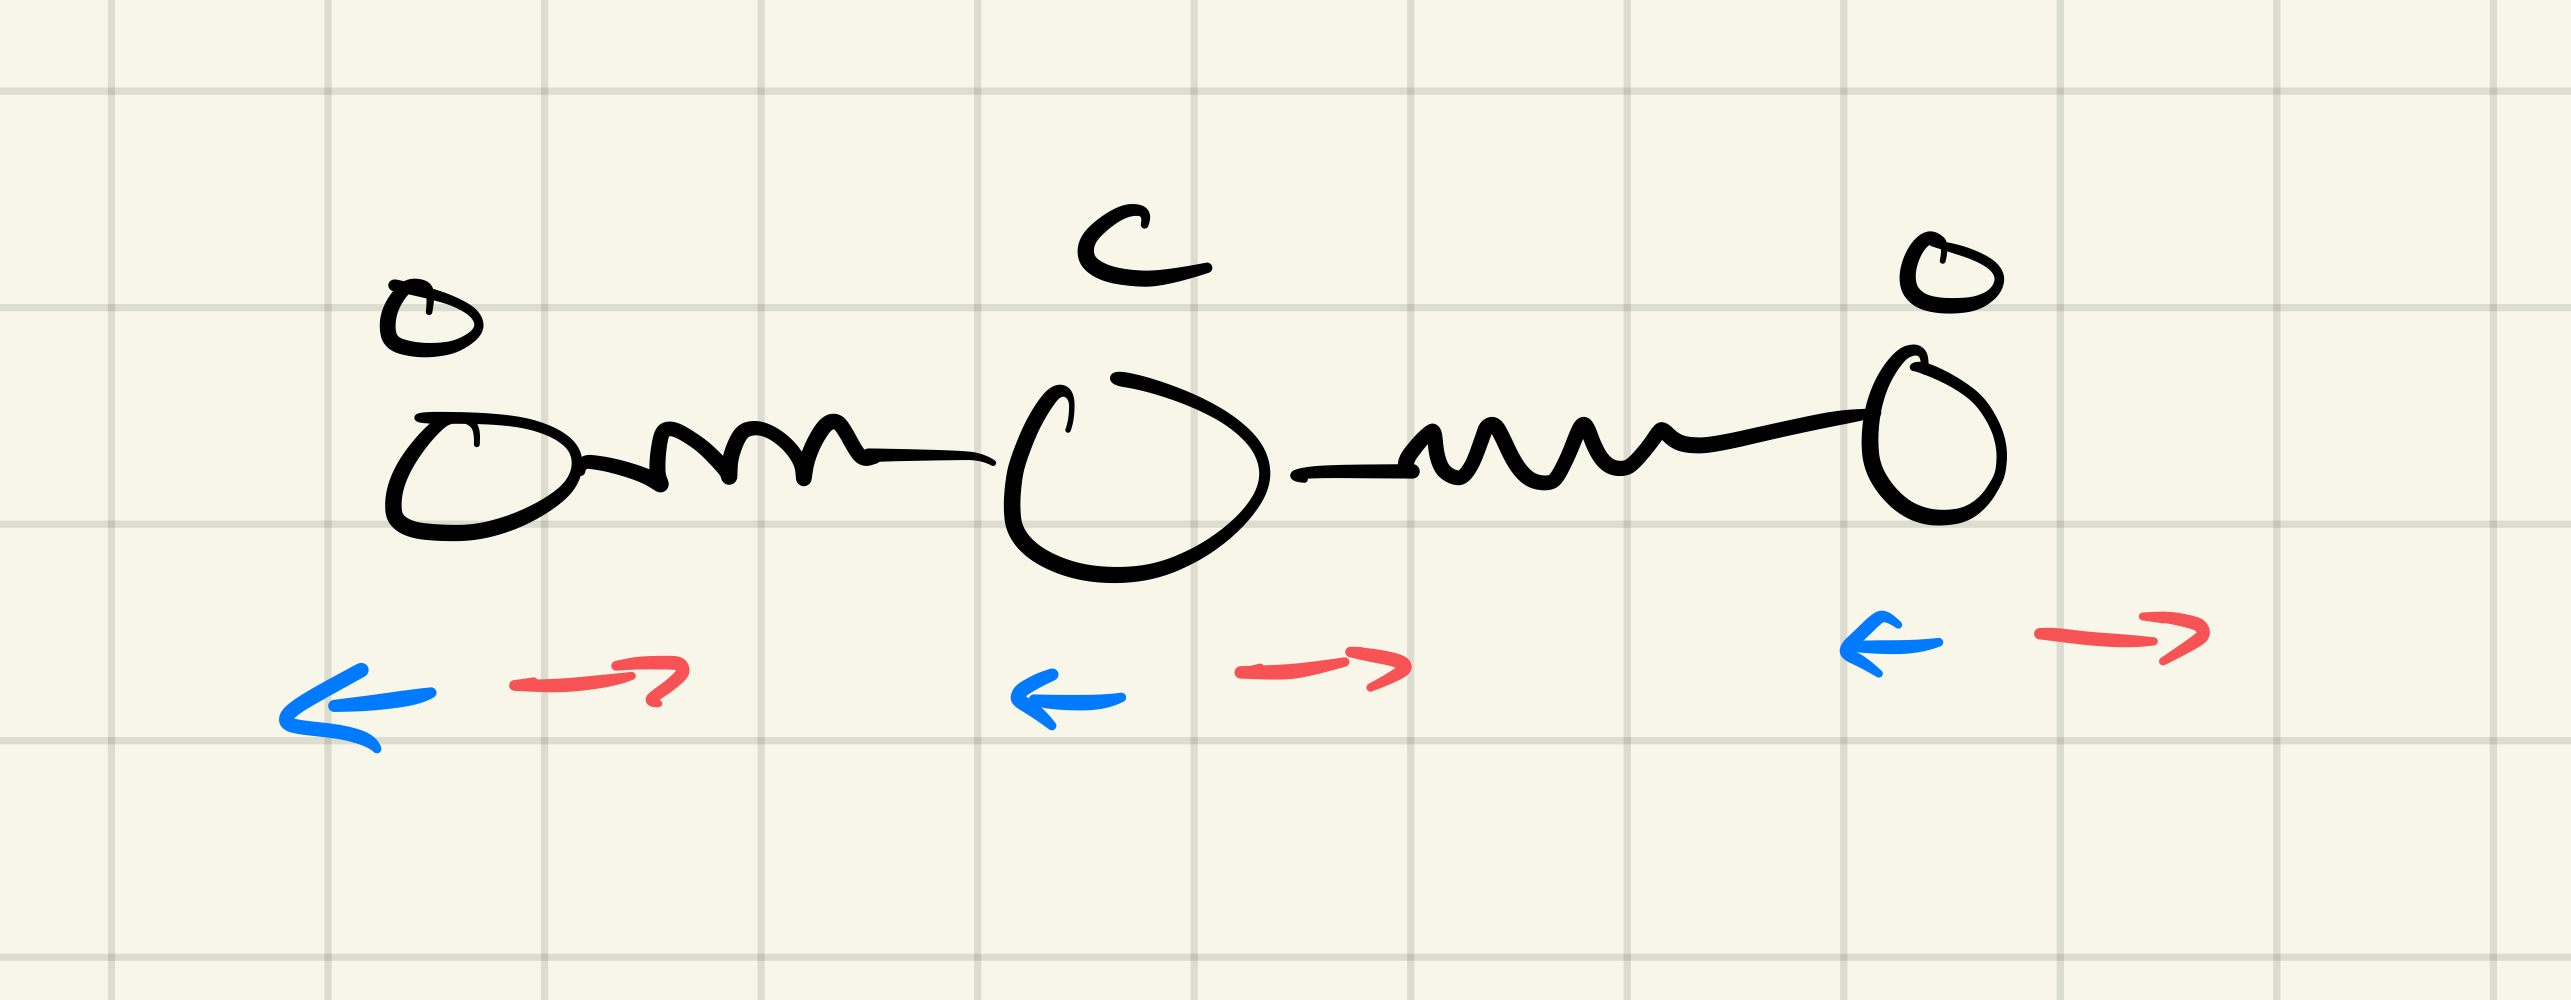
\includegraphics[scale=0.1]{CO2-1.jpeg}
	\end{center}
	Here (and in subsequent diagrams), same colored arrows show the direction of that atom's movement at that
	instant. 

	The second vector $\hat{s}_2$ is a solution where $x_2 = 0$, and $x_1 = -x_3$, meaning that when the leftmost
	oxygen moves to the right, the rightmost oxygen moves to the left while the carbon atom remains 
	stationary. Diagram:

	\begin{center}
		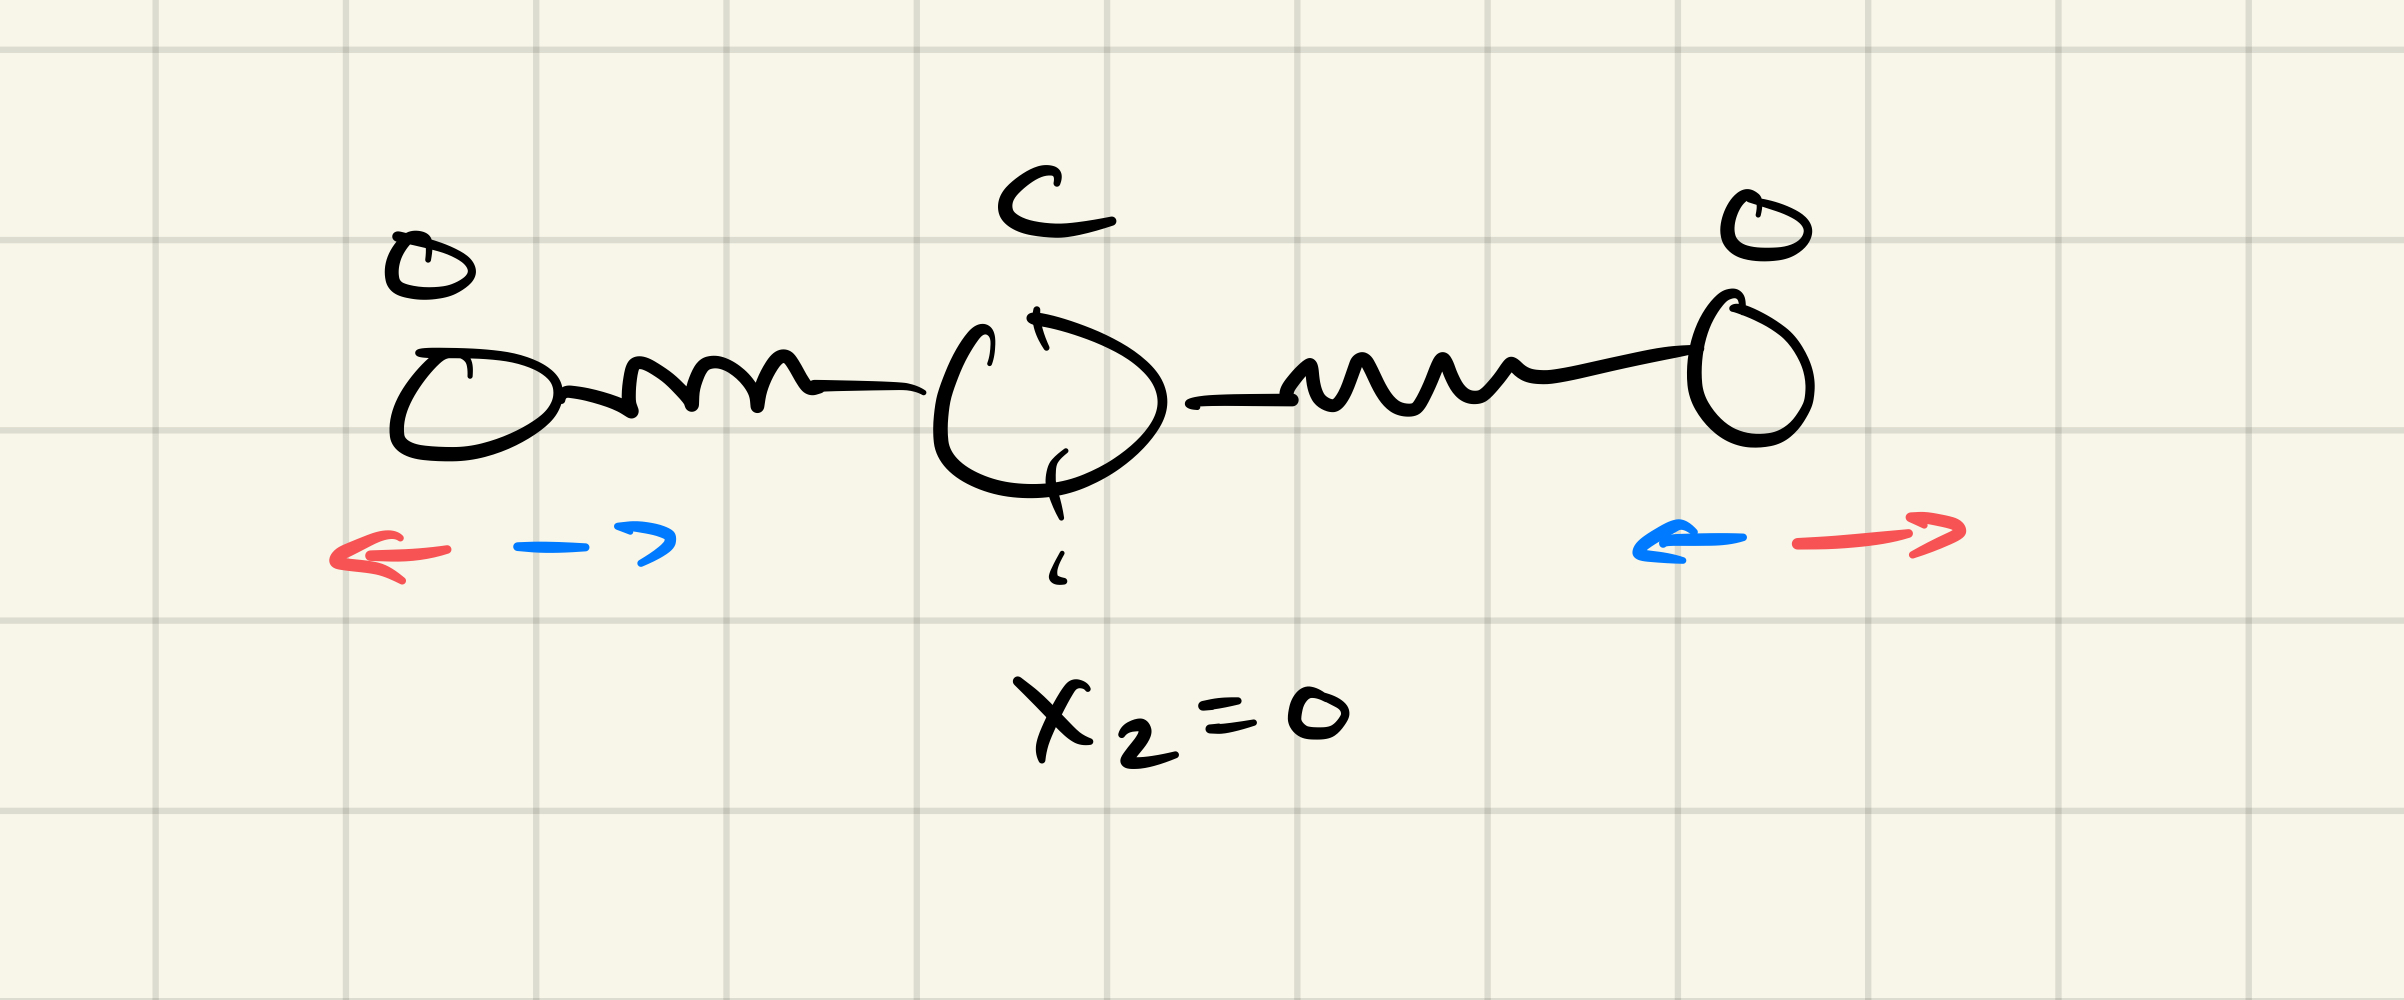
\includegraphics[scale=0.1]{CO2-2.jpeg}
	\end{center}

	Finally, the third vector $\hat{s}_3$ corresponds to the oxygen atoms moving in unison, while the carbon
	atom moves $180^\circ$ out of phase relative to the carbons. Further, the displacement of the oxygen 
	is twice that of the maximum of the individual carbons. Diagram:
	\begin{center}
		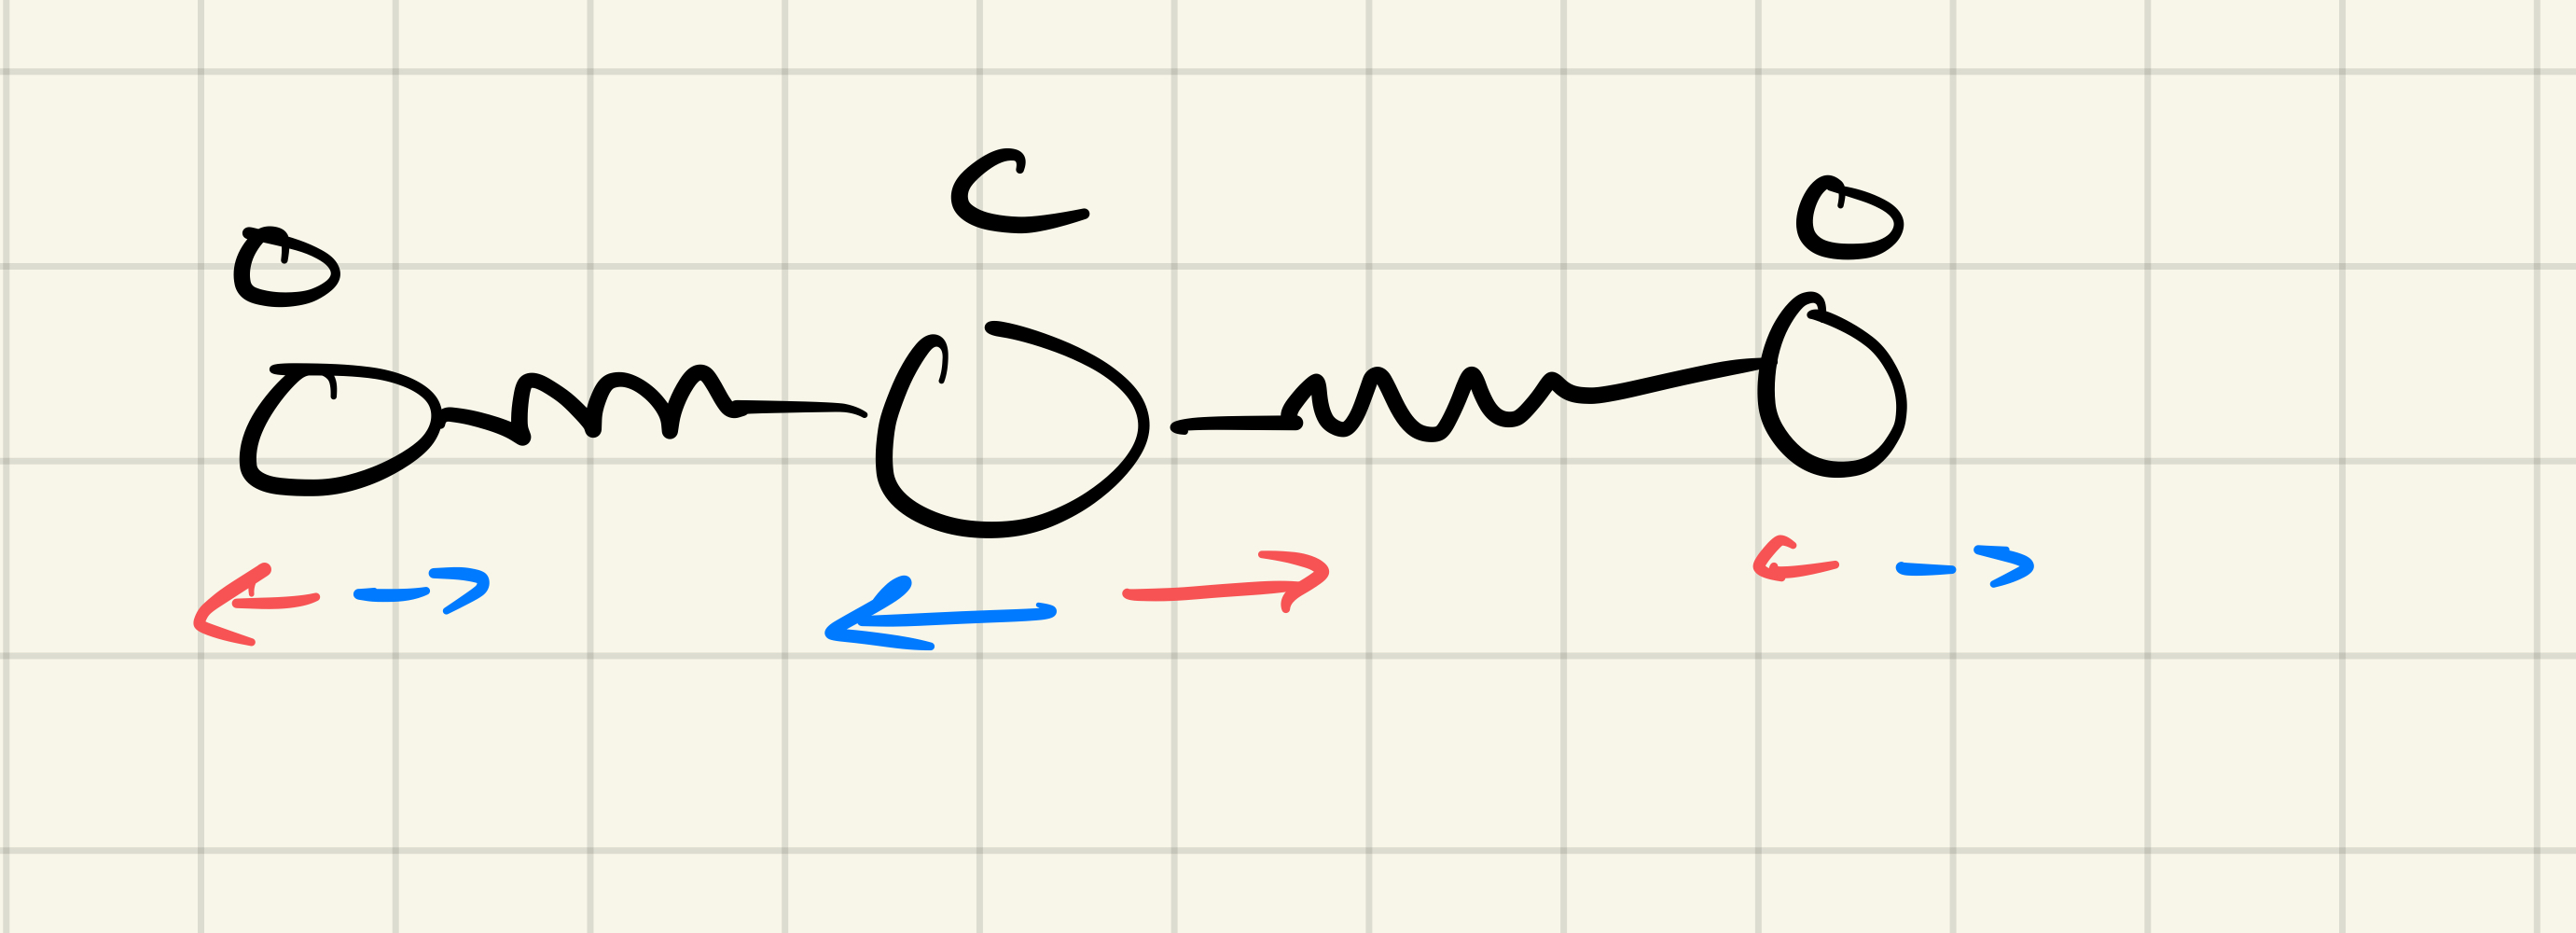
\includegraphics[scale=0.1]{CO2-3.jpeg}
	\end{center}
\end{solution}

\phline
%%%%%%%%%%%%%%%%%%%%%
\paragraph{}
The forces $\vec{F}$ and accelerations $\ddot{\vec{x}}$ for our three particles  can be related by a ``mass matrix'' via $\vec{F} = \mathsf{M}\ddot{\vec{x}}$, with
	\begin{equation*}
		\mathsf{M} = \begin{smpmatrix}{0.8} m_{o} & 0 & 0 \\ 0 & m_{c} & 0 \\ 0 & 0 & m_{o} \end{smpmatrix}.
	\end{equation*}

\paragraph{(e)}		\extrapart
Show that the three original basis unit vectors $\hat{e}_{1}$, $\hat{e}_{2}$, and $\hat{e}_{3}$ are eigenvectors of the mass matrix $\mathsf{M}$.  What are the corresponding
eigenvalues?

\phline
%%%%%%%%%%%%%%%%%%%%%
\paragraph{}
The force vector $\vec{F}$ whose components are the forces on each of the three particles can be found via $\vec{F} = -\vec{\nabla}U$.

\paragraph{(f)}
Show that $\vec{F} = -\mathsf{K}\vec{x}$.  Then use the matrix inverse to solve for $\ddot{\vec{x}}$ in terms of $\vec{x}$ (that is, find the matrix $\mathsf{A}$ such that $\ddot{\vec{x}}
= -\mathsf{A}\vec{x}$).\\
\note{You can make $\mathsf{A}$ prettier by writing $m_{c} = m_{o}/r$, where $r$ is the mass ratio $r = m_{o}/m_{c} = 1.33$.  You can then pull out a factor of
$k/m_{o}$ from the matrix.}

\begin{solution}
	Let $F_i$ be the force on particle $i$. Then, we first compute the gradient:
	\begin{align*}
		F_1 &= -(-k(x_2 - x_1)) = -(kx_1- kx_2)\\
		F_2 &= -k(x_2 - x_1) - k(x_3 - x_2) = -(-kx_1 + 2kx_2 -kx_3) \\
		F_3 &= -k(x_3 - x_2)  = -(-kx_2 + kx_3)
	\end{align*}
	We see that the coefficients of $F_1$ correspond to the first row of the matrix $K$, and the same goes for 
	the other two rows. Therefore, we can actually write:
	\[
	\begin{pmatrix} F_1\\F_2\\F_3 \end{pmatrix} = - \begin{pmatrix}  k & -k & 0\\ -k & 2k & -k\\ 0 & -k & k \end{pmatrix} \begin{pmatrix} x_1\\x_2\\x_3 \end{pmatrix} 
	\] 
	Here, the $3 \times 3$ matrix is incidentally $K$, so therefore we conclude that we can indeed write $\vec F = 
	-K \vec x$
	To find $A$, we use the equation $-K\vec x = M \ddot{\vec x}$. Then, we notice that if we multiply both 
	sides on the left by $M^{-1}$, then we can get the matrix $A$. In other words, we know that $A = M^{-1}K$. 
	First, computing the inverse of $M$, we can compute the cofactor matrix by computing the minors then 
	tacking on the correct sign. Again, we've already had our homework on computing inverses, so I'm going to 
	be brief here. Our cofactor matrix becomes:
	\[
		C_M = \begin{pmatrix} \frac{m_o^2}{r}& 0 & 0\\ 0 & m_o^2 & 0 \\ 0 & 0 & \frac{m_o^2}{r} \end{pmatrix} 
	\] 
	Since $C_M$ is diagonal, then $C_M = C_M^\T$, so we don't have to transpose it. Further, since $M$ is 
	diagonal, its determinant is easy, $\det(M) = m_o^3 / r$. So, we have: 
	\[
		M^{-1} = \frac{C_M^\T}{\det(M)} = \begin{pmatrix} \frac{1}{m_o} &0 &0\\ 0  & \frac{r}{m_o} & 0 \\ 0 &0 & 
		\frac{1}{m_o}\end{pmatrix} 
	\] 
	Now, we are ready to multiply this with $K$:
	\begin{align*}
		A &=  M^{-1}K \\
		  &= \begin{pmatrix} \frac{1}{m_o} & 0 &0\\ 0 & \frac{r}{m_o} & 0 \\ 0 & 0 & \frac{1}{m_o} \end{pmatrix} \begin{pmatrix} k & -k & 0\\ -k & 2k & -k\\ 0 & -k & k \end{pmatrix}  \\
		  &= \begin{pmatrix} \frac{k}{m_o} & -\frac{k}{m_o} & 0\\ -\frac{kr}{m_o} & \frac{2kr}{m_o} & -\frac{kr}{m_o}\\ 0 & -\frac{k}{m_o} & \frac{k}{m_o} \end{pmatrix}
	\end{align*}
\end{solution}



\phline
%%%%%%%%%%%%%%%%%%%%%
\paragraph{}
Since the original basis is an eigenbasis of the mass matrix $\mathsf{M}$ we may call the basis the \heavydef{mass eigenbasis}.  Similarly, since the three vectors 
$\hat{s}_{1}$, $\hat{s}_{2}$, and $\hat{s}_{3}$ form an eigenbasis of the ``spring constant'' matrix $\mathsf{K}$ we may call it the \heavydef{spring eigenbasis}.
We can find orthonormal eigenbases for both of these matrices because they are \heavydef{normal matrices} (recall from Module 4 that a matrix is normal if it
commutes with its Hermitian conjugate.)

%%%%%%%%%%%%%%%%%%%%%
\paragraph{(g)}
Show that $\mathsf{K}$ is a normal matrix but $\mathsf{A}$ is not.

\begin{solution}
	The commutator of two matrices is defined as $[A, B] = AB - BA$. Here, we are asked to show that $K$ commutes
	with its Hermitian conjugate, whereas $A$ does not. First, we note that both are real matrices, so 
	therefore we just need to take the transpose. 

	For $K$, the matrix is symmetric, meaning that it is equal to its transpose. This is nice, since it means 
	that $K K^\T = K^\T K$, hence the commutator $[K, K^\T] = [K, K] = 0$, since we know that any matrix 
	commutes with itself. 
	
	As for $A$, we have to be a bit more mechanical about it:
	\[
		A^\T = \begin{pmatrix} \frac{k}{m_o} & -\frac{kr}{m_o} & 0\\ -\frac{k}{m_o} & \frac{2kr}{m_o} & -\frac{k}{m_o}\\ 0 & -\frac{kr}{m_o} & \frac{k}{m_o } \end{pmatrix} 
	\] 
	Now we compute the commutator terms separately:
	\begin{align*}
		A A^\T &= \begin{pmatrix}  \frac{k}{m_o} & -\frac{k}{m_o} & 0\\ -\frac{kr}{m_o} & \frac{2kr}{m_o} & -\frac{kr}{m_o}\\ 0 & -\frac{k}{m_o} & \frac{k}{m_o} \end{pmatrix} 
		\begin{pmatrix}  \frac{k}{m_o} & -\frac{kr}{m_o} & 0\\ -\frac{k}{m_o} & \frac{2kr}{m_o} & -\frac{k}{m_o}\\ 0 & -\frac{kr}{m_o} & \frac{k}{m_o } \end{pmatrix} \\
&= \frac{k^2}{m_o^2}\begin{pmatrix} 1 & -1 & 0\\-r & -2r & -r\\0 & -1 & 1 \end{pmatrix} \begin{pmatrix} 1 & -r & 0\\ -1 & 2r & -1 \\ 0 & -r & 1 \end{pmatrix}  \\
&= \frac{k^2}{m_o^2}\begin{pmatrix} 2 & -r - 2r & 1 \\-r - 2r & r^2 + 4r + r^2 & -2r - r\\1 & -2r - r & 2  \end{pmatrix}  \\
&= \frac{k^2}{m_o^2}\begin{pmatrix} 2 & -3r & 1 \\ -2r & 6r & -3r\\1 & -3r & 2 \end{pmatrix}  \\
	\end{align*}
	Now for the other one:
	\begin{align*}
		A^\T A &=\begin{pmatrix}  \frac{k}{m_o} & -\frac{kr}{m_o} & 0\\ -\frac{k}{m_o} & \frac{2kr}{m_o} & -\frac{k}{m_o}\\ 0 & -\frac{kr}{m_o} & \frac{k}{m_o } \end{pmatrix} \begin{pmatrix}  \frac{k}{m_o} & -\frac{k}{m_o} & 0\\ -\frac{kr}{m_o} & \frac{2kr}{m_o} & -\frac{kr}{m_o}\\ 0 & -\frac{k}{m_o} & \frac{k}{m_o} \end{pmatrix} 
\\
&= \frac{k^2}{m_o^2}\begin{pmatrix}1 & -r & 0\\ -1 & 2r & -1\\0 & -r & 1  \end{pmatrix} \begin{pmatrix} 1 & -1 & 0\\-r & 2r & -r\\0& -1 & 1 \end{pmatrix}   \\
&= \frac{k^2}{m_o^2}\begin{pmatrix} 1 + r^2 & -1 - 2r^2 & r^2 - 1\\ -1 - r^2 & 1 + 4r + 1 & -2r^2 -1\\
r^2 & -2r^2 - 1 & r^2 + 1\end{pmatrix}  \\
&= \frac{k^2}{m_o^2} \begin{pmatrix} 1 + r^2 & -1 - 2r^2 & r^2 - 1\\ -1 - r^2 &2 + 4r & -2r^2 -1\\
r^2 & -2r^2 - 1 & r^2 + 1\end{pmatrix}
	\end{align*}
	Clearly, these two matrices are not equal to one another, so therefore $A$ is not a normal matrix.
	\footnote{It was only after the fact that someone told me all I had to do was compute one element of the 
	matrix. Oh well, it's all written up already}
\end{solution}


\bigskip
\dphline
\pagebreak
%%%%%%%%%%%%%%%%%%%%%%%%%%%%%%%%%%%%%%%%%%%%%%%%%%%%%%%%%%%%%%%%%%%%%%%%%%%%%%%%
\section*{Problem 5.3 - Eigenproofs!}
\relevid{Projections; 
Eigenproperties of Hermitian, Orthogonal, and Unitary Matrices;  
Eigenvalue and Eigenvector Properties and Theorems}

\paragraph{}
This problem involves proofs about eigenvalues and eigenvectors \emph{and} are the characteristic types of questions I like to ask about eigenvalues and eigenvectors.  The title
``eigenproofs'' takes on a double-meaning!\footnote{Huzzah.  Let's get on with the question, shall we?}

%%%%%%%%%%%%%%%%%%%%%
\paragraph{(a)}
Prove that two eigenvectors belonging to different eigenspaces are linearly independent of each other.

\begin{solution}
	Suppose we have two (nonzero) vectors $\vec v_1,\vec v_2$ with $A\vec v_1 = \lambda_1 v_1$ and $A \vec v_2 = 
	\lambda_2 \vec v_2$, and $\lambda_1 \neq \lambda_2$. In order for the eigenvectors to be linearly 
	independent, we simply need to show that $\vec v_1$ cannot be written as a scalar multiple of $\vec v_2$. 
	Suppose by contradiction that $\vec v_1 = k \vec v_2$. Then, we have $A \vec v_1 = \lambda_1 \vec v_1$, 
	and also $A(k \vec v_2) = k \lambda_2 \vec v_2$. This implies that:
	\[
	\lambda_1 \vec v_1 = k \lambda_2 \vec v_2 
	\] 
	Now rearranging:
	\begin{align*}
		\lambda_1 \vec v_1 - k\lambda_2\vec v_2 &= \vec 0\\
		\lambda_1 \vec v_1 - \lambda_2(\underbrace{k \vec v_2}_{= \vec v_1}) &= \vec 0\\
		\therefore \vec v_1(\lambda_1 - \lambda_2) &= \vec 0
	\end{align*}
	And since $\vec v_1$ is assumed to be nonzero, then we can only conclude that $\lambda_1 = \lambda_2$, but 
	this is a contradiction to the fact that the eigenvalues are distinct. Hence, eigenvectors belonging 
	to different eigespaces are linearly independent. 
\end{solution}

%%%%%%%%%%%%%%%%%%%%%
\paragraph{(b)}
Prove that if $\vec{v}$ is an eigenvector of an invertible matrix $\mathsf{M}$ belonging to eigenvalue $\lambda$ then it is also an eigenvector of $\mathsf{M}^{-1}$.  
Find the associated eigenvalue.

\begin{solution}
	Since we know that $\vec v$ is an eigenvector, we can write:
	\[
	M \vec v = \lambda \vec v
	\] 
	Now multiply by $M^{-1}$ on the left of both equations:
	\begin{align*}
		\underbrace{M^{-1}M}_{= \mathbbold 1} \vec v &= M^{-1}\lambda \vec v\\
		\vec v &= \lambda M^{-1} \vec v \\
		\therefore \frac{1}{\lambda}\vec v &= M^{-1} \vec v 
	\end{align*}
	This is an eigenvalue equation with $\vec v$ as the eigenvector and associated eigenvalue of 
	$\frac{1}{\lambda}$.
\end{solution}

%%%%%%%%%%%%%%%%%%%%%
\paragraph{(c)}
Prove that the eigenvalues of a unitary matrix $\mathsf{U}$ (and thus also real orthogonal matrices) all lie on the unit circle in the complex plane.  That is, the eigenvalues
all satisfy $\abs{\lambda} = 1$.
\spoilers{Let $\vec{v}$ be an eigenvector of $\mathsf{U}$ and consider the combination $\vec{v}^{\t}\mathsf{U}^{\t}\mathsf{U}\vec{v}$.}

\begin{solution}
	This was done in lecture. Let $\vec v$ be an eigenvector of $U$, and now we square both sides:
	\begin{align*}
		(U \vec v) \cdot (U \vec v) = (U\vec v)^\dagger U \vec v = \vec v^\dagger U^\dagger U \vec v = |v|^2
	\end{align*}
	On the right hand side we have:
	\[
		(\lambda v) \cdot (\lambda v) = \lambda \lambda^* \vec v^\dagger \vec v = |\lambda|^2 |v|^2
	\] 
	so we have the equation $|\lambda|^2 |\vec v^2| = |\vec v^2|$, implying that $|\lambda|^2 = 1$. Taking 
	the square root, this implies that $|\lambda| = 1$, as desired. Consequently, this means that all 
	eigenvalues of $U$ occupy a unit circle on the complex plane, since those are the only vectors with 
	magnitude 1. 
\end{solution}

%%%%%%%%%%%%%%%%%%%%%
\paragraph{(d)}		\extrapart
Show that the eigenvalues of an anti-Hermitian matrix are all purely imaginary.


%%%%%%%%%%%%%%%%%%%%%
\paragraph{(e)}		\extrapart
Show that the eigenvalues of a diagonal matrix are the diagonal elements.  Then show the same thing for upper-triangular matrices.


%%%%%%%%%%%%%%%%%%%%%
\paragraph{(f)}
Prove that if $\vec{v}$ is an eigenvector of a matrix $\mathsf{M}$ belonging to eigenvalue $\lambda$ then $\mathsf{S}^{-1}\vec{v}$ is an eigenvector of the matrix 
$\widetilde{\mathsf{M}}\equiv \mathsf{S}^{-1}\mathsf{MS}$ belonging to the same eigenvalue $\lambda$.\\
\note{This is known as a \heavydef{similarity transformation}, which we will learn more about in Module 6.}

\begin{solution}
	To do this we just act $\tilde M$ on $S^{-1}\vec v$:
	\begin{align*}
		\tilde M S^{-1} \vec v &= (S^{-1}MS) S^{-1} \vec v\\	
							   &= S^{-1} M (S S^{-1}) \vec v \\
							   &= S^{-1}M \vec v \\
							   &= S^{-1} \lambda \vec v \\
							   &= \lambda S^{-1} \vec v
	\end{align*}
	This is the eigenvalue equation for $\tilde M$, with $\lambda$ as the eigenvalue, and $S^{-1} \vec v$ 
	as the eigenvector.
\end{solution}

\phline
%%%%%%%%%%%%%%%%%%%%%
\paragraph{}
One of the nice features of having an orthonormal basis (including an eigenbasis) is the \heavydef{resolution of the identity}, which is a special way of writing the identity 
matrix,\footnote{If we are just dealing with real basis vectors the Hermitian conjugate can be replaced by a transpose.}
	\begin{equation}
		\mathbbold{1} = \sum_{i} \hat{e}_{i}\hat{e}_{i}^{\t}.
	\label{resolutionoftheidentity}
	\end{equation}
Furthermore, if $\{\hat{e}_{i}\}$ is an orthonormal eigenbasis for a matrix $\mathsf{M}$ with $\hat{e}_{i}$ belonging to eigenvalue $\lambda_{i}$, 
then we can write $\mathsf{M}$ using the \heavydef{spectral decomposition},
	\begin{equation}
		\mathsf{M} = \sum_{i} \lambda_{i}\hat{e}_{i}\hat{e}_{i}^{\t}.
	\label{spectraldecomposition}
	\end{equation}
Consider the rotation matrix $\mathsf{R}_{\theta} \equiv \smmatrix{1}{\cos\theta & -\sin\theta \\ \sin\theta & \cos\theta}$.


%%%%%%%%%%%%%%%%%%%%%
\paragraph{(g)}		\extrapart
Show from scratch that $\mathsf{R}_{\theta}$ has eigenvalues $e^{i\theta}$ and $e^{-i\theta}$ with
corresponding orthonormal eigenbasis $\left\{\sqrtfinv{2}\smtwovect{1}{-i},\sqrtfinv{2}\smtwovect{1}{i}\right\}$.


%%%%%%%%%%%%%%%%%%%%%
\paragraph{(h)}
Using the eigenbasis described in the previous part, verify Eqs.~\ref{resolutionoftheidentity} and~\ref{spectraldecomposition}.

\begin{solution}
	We can just mechanically compute the sum:
	\begin{align*}
		e_1e_1^\dagger + e_2e_2^\dagger &=\frac{1}{2} \begin{pmatrix}1 \\ -i \end{pmatrix}
		\begin{pmatrix} 1 & i \end{pmatrix} + \frac{1}{2}\begin{pmatrix} 1\\i \end{pmatrix} 
		\begin{pmatrix} 1 & -i \end{pmatrix} \\
						  &= \frac{1}{2}\begin{pmatrix} 1 & i \\ -i & 1 \end{pmatrix} + \frac{1}{2}
		\begin{pmatrix} 1 & -i \\ i & 1 \end{pmatrix}  \\
						  &= \frac{1}{2}\begin{pmatrix} 2 & 0 \\ 0 & 2 \end{pmatrix} \\
									   &= \begin{pmatrix} 1 & 0 \\ 0 & 1 \end{pmatrix}  
	\end{align*} 
	As for equation 2, we have:
	\begin{align*}
		M &= e^{i \theta} e_1 e_1^\dagger + e^{-i \theta} e_2e_2^\dagger \\
		  &= e^{i \theta} \frac{1}{2}\begin{pmatrix} 1&i \\ -i & 1 \end{pmatrix} + \frac{1}{2}e^{i \theta}
		\begin{pmatrix} 1 & -i\\ i & 1 \end{pmatrix} \\
						  &= \begin{pmatrix} \frac{e^{i \theta} + e^{- i \theta}}{2} & 
						  \frac{i(e^{i \theta} - e^{- i \theta})}{2}\\
					  \frac{i(e^{- i \theta} - e^{i \theta})}{2}& 
				  \frac{e^{i \theta} + e^{- i \theta}}{2}\end{pmatrix}
	\end{align*}
	Here we remember our exponential identities. For the top right entry, we can write it as:
	\[
		\frac{i(e^{- i \theta} - e^{- i \theta})}{2} \cdot \frac{i}{i} = -\frac{e^{i \theta} - e^{- i \theta}}{2i}
		 = - \sin \theta 
	\] 
	For the bottom left entry, we have:
	\[
		\frac{i(e^{- i \theta} - e^{i \theta})}{2} \cdot \frac{i}{i} = -\frac{e^{-i \theta} - e^{i \theta}}{2}
		= \frac{e^{i \theta} - e^{- i \theta}}{2i} = \sin \theta 
	\] 
	The diagonal terms are just the standard cosine identity. Therefore we have:
	\[
		M = \begin{pmatrix} \cos \theta & - \sin \theta\\ \sin \theta & \cos \theta  \end{pmatrix} 
	\] 
	as desired.
\end{solution}

\bigskip
\dphline
\pagebreak
%%%%%%%%%%%%%%%%%%%%%%%%%%%%%%%%%%%%%%%%%%%%%%%%%%%%%%%%%%%%%%%%%%%%%%%%%%%%%%%%
\section*{Problem 5.4 - Waves on a String (Plus Review)}

In Problem 2.4, we considered the vector space of the shapes that a string stretched between $x=0$ and $x=L$ can take, with the vectors in this space
being represented by functions $\vec{f} \doteq f(x)$ with $f(0)=f(L)=0$.  If our string is held under tension $T$ and has a lineal mass density $\rho$ (mass-per-unit-length) then
the equation of motion for the string is given by a \heavydef{wave equation},\footnote{We will study the wave equation in Module 10.}
	\begin{equation}
		\frac{\partial^{2}f(x,t)}{\partial t^{2}} = \frac{T}{\rho}\,\frac{\partial^{2}f(x,t)}{\partial x^{2}}.
	\label{waveequation}
	\end{equation}
We can write this in matrix language just like we did in our masses-on-a-spring example,\footnote{In fact, this may be considered the ``continuous'' version of that
system.}
	\begin{equation*}
		\frac{d^{2}{\vec{f}}}{dt^{2}} = \mathsf{W}\vec{f}(t),
	\end{equation*}
where $\mathsf{W}$ is a linear transformation on our vector space of shapes on a string defined via
	\begin{equation*}
		\vec{f} \doteq	f(x)	\eqimplies \mathsf{W}\vec{f} \doteq \frac{T}{\rho}\,\frac{\partial^{2}f(x)}{\partial x^{2}}.
	\end{equation*}
This transformation is proportional to the \heavydef{Laplacian}.


%%%%%%%%%%%%%%%%%%%%%
\paragraph{(a)}		\reviewpart
Show that $\mathsf{W}$ is indeed a linear transformation.


\phline
%%%%%%%%%%%%%%%%%%%%%
\paragraph{}	
Since $\mathsf{W}$ is a linear transformation, we can apply a lot of our matrix ideas to it!  First, recall that our inner/scalar/dot product for this vector space (assuming
all of our functions are real) is
	\begin{equation*}
		\vec{f}\cdot\vec{g} = \int_{0}^{L}\!f(x)\,g(x)\, dx.
	\end{equation*}
A \heavydef{self-adjoint} transformation $\mathsf{H}$ is the linear transformation version of a Hermitian matrix, $\mathsf{H}^{\t}=\mathsf{H}$.  In particular, this means
	\begin{equation*}
		\vec{f}\cdot(\mathsf{H}\vec{g}) = (\mathsf{H}^{\t}\vec{f})\cdot\vec{g} = (\mathsf{H}\vec{f})\cdot\vec{g}.
	\end{equation*}

%%%%%%%%%%%%%%%%%%%%%
\paragraph{(b)}		\reviewpart
Show that $\mathsf{W}$ is self-adjoint.  Use vectors/functions $\vec{f}\doteq f(x)$ and $\vec{g} \doteq g(x)$ with boundary conditions $f(0)=g(0)=f(L)=g(L) = 0$ for this.
\spoilers{You will need to use integration by parts twice!}



\phline
%%%%%%%%%%%%%%%%%%%%%
\paragraph{}
Since $\mathsf{W}$ is Hermitian we know that it has real eigenvalues and its eigenvectors are orthogonal.  The eigenvalue equation as always reads
$\mathsf{W}\vec{f} = \lambda\vec{f}$.  Finding eigenvalues and eigenvectors for infinite-dimensional vector spaces (such as our shapes-on-a-string
vector space) is not as straightforward as it was when we had actual matrices.  We have to brute-force it by actually solving the differential equation.\footnote{This is a preview of Module 8.}


%%%%%%%%%%%%%%%%%%%%%
\paragraph{(c)}
Show that the ``trial solution'' $\vec{f}\doteq A\cos(kx) + B \sin(kx)$ solves the eigenvalue equation.  What is the associated eigenvalue?
What restrictions must be put on $A$, $B$, and/or $k$ in order for $\vec{f}$ to satisfy the boundary conditions $f(0)=f(L)=0$?.
\spoilers{Partial answer: $k = n\pi/L$ with $n\in\mathbb{Z}$.}

\begin{solution}
	Acting $W$ on $\vec f$:
	\begin{align*}
		W \vec f &= \frac{T}{\rho}\pdv[2]{x}(A \cos(kx) + B \sin (kx))\\
		&= \frac{T}{\rho}\left(-Ak^2 \cos(kx) - Bk^2\sin(kx)\right) \\
		&= -\frac{Tk^2}{\rho}\underbrace{(A \cos(kx) - B\sin(kx))}_{\vec f} 
	\end{align*}
	This is exactly the eigenvalue equation, which is what we wanted to show. Here, our associated eigenvalue is
	$\lambda = -\frac{Tk^2}{\rho}$. As for restrictions, $f(0) = 0$ immediately 
	deletes any cosine term, so we're forced to conclude that $A = 0$. As for $f(L) = 0$, this means that 
	we must be at an integer multiple of $\pi$ when $x = L$. The only way to guarantee that is if we let 
	$k = n\pi / L$ where $n$ is any integer. There are no restrictions on $B$. Thus, our function looks like:
	\[
	\vec f_n = B\sin(\frac{n \pi x}{L})
	\] 
\end{solution}
\phline
%%%%%%%%%%%%%%%%%%%%%
\paragraph{} 
The boundary conditions mean we can only find non-trivial eigenvectors when $k=n\pi/L$, where $n$ is an integer.  We are thus left with a set of eigenvalues and eigenvectors 
indexed by the integer $n$.  We will call the normalized vectors $\{\hat{e}_{n}\}$ and the corresponding eigenvalues $\lambda_{n}$.

\paragraph{(d)}
Show that $n=0$ gives a trivial solution and can thus be ignored.  For $n\neq 0$, normalize the eigenvectors to create the set $\{\hat{e}_{n}\}$.  Show that
$\hat{e}_{-n}$ is proportional to $\hat{e}_{+n}$.  This means we can restrict $n$ to the natural numbers $\mathbb{N}$, $n=1,2,\cdots$.
Verify that the remaining eigenvectors $\{\hat{e}_{n}\}$ with $n\in\mathbb{N}$ are orthogonal.
We have created an orthonormal basis for shapes on a string!

\begin{solution}
	As for $n = 0$, we see that $\sin(0) = 0$, so therefore $\hat{e}_0 = 0$, which is a trivial solution. For
	the normalization condition, we want $\hat{e}_n \cdot \hat{e}_n = 1$, so therefore this means we want:
	\[
	B^2 \int_0^L \sin^2\left(\frac{n \pi x}{L}\right) dx = 1
	\] 
	This integral can be computed by hand using double angle identities, but since we're allowed mathematica here
	I just threw it in there and we get that the integral evaluates to $L / 2$. Therefore:
	\[
	B^2 \left(\frac{L}{2}\right) = 1 \implies B = \sqrt{\frac{2}{L}} 
	\] 
	which is our normalization condition. Now we show that $\hat{e}_{+n}$ is proportional to $\hat{e}_{-n}$. To
	do this, let's look at $\hat{e}_{+n}$:
	\[
		\hat{e}_{+n} = \sqrt{\frac{2}{L}}  \sin(\frac{n \pi x}{L})
	\] 
	And $\hat{e}_{-n}$:
	\[
		\hat{e}_{-n} = \sqrt{\frac{2}{L}}  \sin(-\frac{n \pi x}{L})
	\] 
	Now we use the fact that the sine function is odd, so $\sin(-x) = -\sin(x)$. So we can take the negative
	out of the argument:
	\[
		\hat{e}_{-n} = -\sqrt{\frac{2}{L}}  \sin(\frac{n \pi x}{L}) = -\hat{e}_{+n}
	\] 
	hence we've proven proportionality. As for orthogonality, we have to show that $\hat{e}_n \cdot \hat{e}_m = 
	\delta_{nm}$, which is the condition for orthogonality. We actually did this explicitly in problem 2.4, where
	we showed that:
	\[
	\frac{2}{L}\int_0^L \sin\left(\frac{n \pi x}{L}\right)
	\sin\left( \frac{m \pi x}{L}\right) dx = \delta_{nm}
	\] 
	It turns out that $\hat{e}_n \cdot \hat{e}_m$ is exactly the left hand side (by definition of the inner 
	product on this vector space), so we have $\hat{e}_n \cdot \hat{e}_m
	= \delta_{nm}$, which is exactly the definition of orthogonality. 
\end{solution}

\phline
%%%%%%%%%%%%%%%%%%%%%
\paragraph{}
The physical significance of the eigenvectors is that they are the \heavydef{standing waves} on the string!  Define $\omega_{n} \equiv \sqrt{\abs{\lambda_{n}}}$ so that
the wave equation Eq.~\ref{waveequation} becomes the standing wave equation,
	\begin{equation}
		\ddot{\vec{f}}_{n} = -\omega^{2}_{n}\vec{f}_{n}.
	\label{standingwaveequation}
	\end{equation}


%%%%%%%%%%%%%%%%%%%%%
\paragraph{(e)}
Show that $\vec{f}_{n}(t) = C \cos(\omega_{n} t)\hat{e}_{n}$ solves the standing wave equation Eq.~\ref{standingwaveequation}.  
Thus we see that the eigenvalues are related to the squares of the \heavydef{frequencies} of the standing waves.

\begin{solution}
	Plug and chug to verify:
	\begin{align*}
		\ddot{\vec f}_n(t) &= \pdv[2]{t}\left( C \cos(\omega_nt) \sqrt{\frac{2}{L}}  \sin\left( \frac{n \pi x}{L}\right)\right)\\
					   &= C\sqrt{\frac{2}{L}}  \sin\left(\frac{n \pi x}{L}\right) \pdv[2]{t}\cos(\omega_nt) \\
						   &= -C\sqrt{\frac{2}{L}} \sin\left(\frac{n \pi x}{L}\right) \omega_n^2 \cos(\omega_n t) \\
						   &= -\omega_n^2 \underbrace{\left(C \cos(\omega_n t)
						   \sqrt{\frac{2}{L}}  \sin(\frac{n \pi x}{L})\right)}_{\vec f_n} \\
						   &= -\omega_n^2 \vec f_n 
	\end{align*} 
	as desired. 
\end{solution}

\phline
%%%%%%%%%%%%%%%%%%%%%%%%%%%%%%%%%%%%%%%%%%%%%%%%%%%%%%%%%%%%%%%%%%%%%%%%%%%%%%%%
\paragraph{}
The rest of this problem is left as a ``challenge'' problem to stretch yourself and preview the future of the course and is not for credit.

%%%%%%%%%%%%%%%%%%%%%
\paragraph{(f)}		\extrapart
More generally, let the initial shape of the string be described by $\vec{f}_{0} = \sum_{n=1}^{\infty} c_{n}\hat{e}_{n}$ and let the string be released from rest.
Show that the time-evolution for the string (the ``wave'') is then given by $f(x,t) = \sum_{n=1}^{\infty} c_{n}\cos(\omega_{n}t){e}_{n}(x)$,
where $\hat{e}_{n}\doteq e_{n}(x)$.

\paragraph{(g)}		\extrapart
Use the result from part (f), your expansion of the triangle wave from Problem 2.4(d), and a graphing program such as Python or Mathematica to create an animation of the 
triangle wave on a string.\\
\note{You may need to non-dimensionalize - that is, define new dimensionless length and time variables to properly plot things.  This is equivalent to setting $L=1$
and $\omega_{1}=1$.  You should also introduce a cutoff on the sum.  Ten terms gives a nice sharp initial triangle.}


\endofhomework
\addfooter
%%%%%%%%%%%%%%%%%%%%%%%%%%%%%%%%%%%%%%%%%%%%%%%%%%%%%%%%%%%%%%%%%%%%%%%%%%%%%%%%
\end{document}


